\documentclass{article}
\usepackage{graphicx}
\usepackage[utf8]{inputenc}
\usepackage{listings}
\usepackage{color}
\usepackage{xcolor}
\usepackage{textcomp}
\usepackage{amsmath}
\usepackage{mathabx}


\begin{document}

\title{Tarea Polinomio interpolante de newton}
\author{Angel Caceres Licona}

\maketitle

\section{Aproxime $f(8.4$)...}

Para el polinomio de primer grado tenemos la siguiente gráfica:
\begin{center}
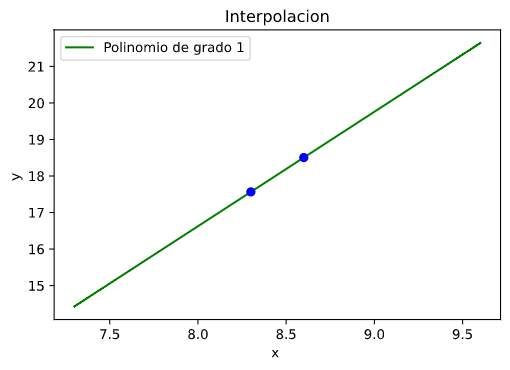
\includegraphics[scale=0.75]{grafica1-1.png}
\end{center}
El valor calculado es 17.8783\\

Para el polinomio de segundo grado tenemos la siguiente gráfica:
\begin{center}
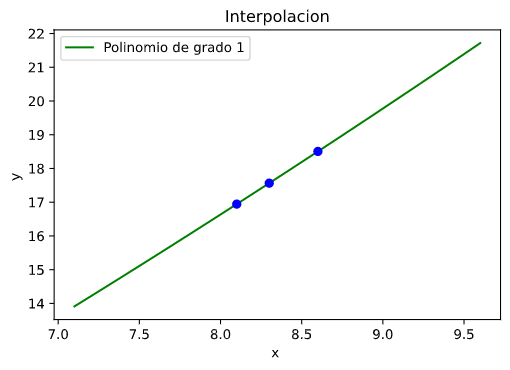
\includegraphics[scale=0.75]{grafica1-2.png}
\end{center}
El valor calculado es 17.8771\\

Para el polinomio de tercer grado tenemos la siguiente gráfica:
\begin{center}
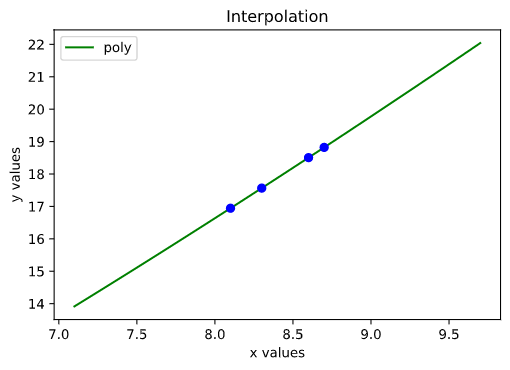
\includegraphics[scale=0.75]{grafica1-3.png}
\end{center}
El valor calculado es 17.8771
\section{Aproxime $f(-1/3)$...}
Para el polinomio de primer grado tenemos la siguiente gráfica:
\begin{center}
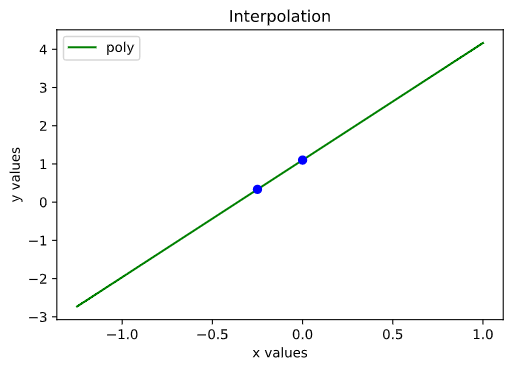
\includegraphics[scale=0.75]{grafica2-1.png}
\end{center}
El valor calculado es 0.215042\\

Para el polinomio de segundo grado tenemos la siguiente gráfica:
\begin{center}
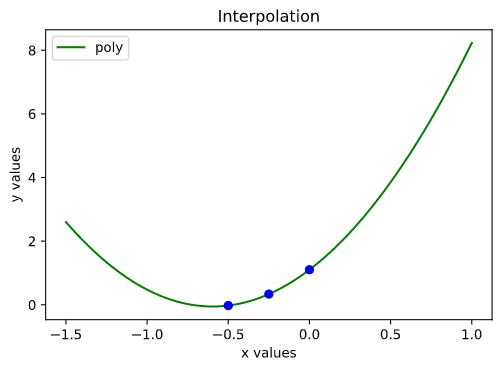
\includegraphics[scale=0.75]{grafica2-2.png}
\end{center}
El valor calculado es 0.169889\\

Para el polinomio de tercer grado tenemos la siguiente gráfica:
\begin{center}
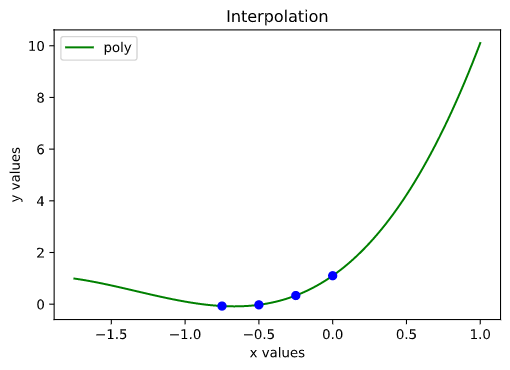
\includegraphics[scale=0.75]{grafica2-3.png}
\end{center}
El valor calculado es 0.174519

\section{Construya el polinomio interpolante...}
Obtenemos el polinomio cuya gráfica es:
\begin{center}
    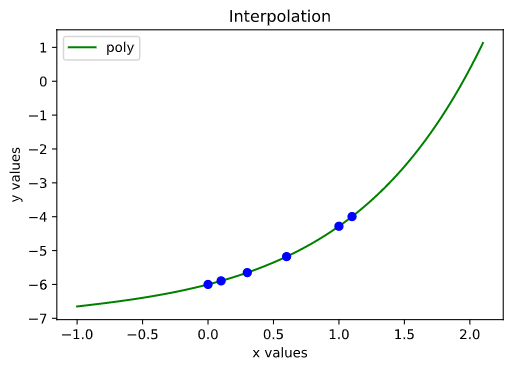
\includegraphics[scale=0.75]{grafica3.png}
\end{center}
\section{Para una función $f$, el polinomio interpolante...}
El resultado obtenido es 6.
\section{Use los datos de la tabla...}
Obtenemos el polinomio cuya gráfica es:
\begin{center}
    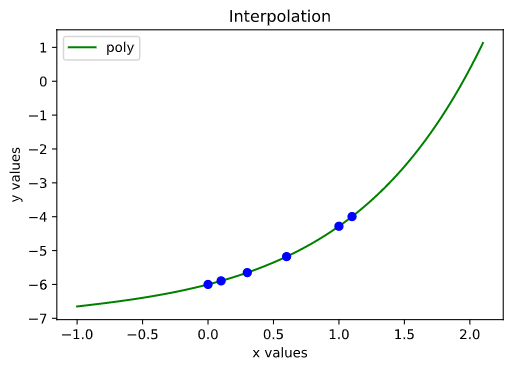
\includegraphics[scale=0.75]{grafica3.png}
\end{center}

Y para $f(0.05)$ obtenemos la siguiente aproximación: -5.94871

\end{document}